%<dscrpt>Fichier de déclarations Latex à inclure au début d'un élément de cours.</dscrpt>

\documentclass[a4paper]{article}
\usepackage[hmargin={1.8cm,1.8cm},vmargin={2.4cm,2.4cm},headheight=13.1pt]{geometry}

%includeheadfoot,scale=1.1,centering,hoffset=-0.5cm,
\usepackage[pdftex]{graphicx,color}
\usepackage[french]{babel}
%\selectlanguage{french}
\addto\captionsfrench{
  \def\contentsname{Plan}
}
\usepackage{fancyhdr}
\usepackage{floatflt}
\usepackage{amsmath}
\usepackage{amssymb}
\usepackage{amsthm}
\usepackage{stmaryrd}
%\usepackage{ucs}
\usepackage[utf8]{inputenc}
%\usepackage[latin1]{inputenc}
\usepackage[T1]{fontenc}


\usepackage{titletoc}
%\contentsmargin{2.55em}
\dottedcontents{section}[2.5em]{}{1.8em}{1pc}
\dottedcontents{subsection}[3.5em]{}{1.2em}{1pc}
\dottedcontents{subsubsection}[5em]{}{1em}{1pc}

\usepackage[pdftex,colorlinks={true},urlcolor={blue},pdfauthor={remy Nicolai},bookmarks={true}]{hyperref}
\usepackage{makeidx}

\usepackage{multicol}
\usepackage{multirow}
\usepackage{wrapfig}
\usepackage{array}
\usepackage{subfig}


%\usepackage{tikz}
%\usetikzlibrary{calc, shapes, backgrounds}
%pour la présentation du pseudo-code
% !!!!!!!!!!!!!!      le package n'est pas présent sur le serveur sous fedora 16 !!!!!!!!!!!!!!!!!!!!!!!!
%\usepackage[french,ruled,vlined]{algorithm2e}

%pr{\'e}sentation du compteur de niveau 2 dans les listes
\makeatletter
\renewcommand{\labelenumii}{\theenumii.}
\renewcommand{\thesection}{\Roman{section}.}
\renewcommand{\thesubsection}{\arabic{subsection}.}
\renewcommand{\thesubsubsection}{\arabic{subsubsection}.}
\makeatother


%dimension des pages, en-t{\^e}te et bas de page
%\pdfpagewidth=20cm
%\pdfpageheight=14cm
%   \setlength{\oddsidemargin}{-2cm}
%   \setlength{\voffset}{-1.5cm}
%   \setlength{\textheight}{12cm}
%   \setlength{\textwidth}{25.2cm}
   \columnsep=1cm
   \columnseprule=0.5pt

%En tete et pied de page
\pagestyle{fancy}
\lhead{MPSI-\'Eléments de cours}
\rhead{\today}
%\rhead{25/11/05}
\lfoot{\tiny{Cette création est mise à disposition selon le Contrat\\ Paternité-Pas d'utilisations commerciale-Partage des Conditions Initiales à l'Identique 2.0 France\\ disponible en ligne http://creativecommons.org/licenses/by-nc-sa/2.0/fr/
} }
\rfoot{\tiny{Rémy Nicolai \jobname}}


\newcommand{\baseurl}{http://back.maquisdoc.net/data/cours\_nicolair/}
\newcommand{\urlexo}{http://back.maquisdoc.net/data/exos_nicolair/}
\newcommand{\urlcours}{https://maquisdoc-math.fra1.digitaloceanspaces.com/}

\newcommand{\N}{\mathbb{N}}
\newcommand{\Z}{\mathbb{Z}}
\newcommand{\C}{\mathbb{C}}
\newcommand{\R}{\mathbb{R}}
\newcommand{\D}{\mathbb{D}}
\newcommand{\K}{\mathbf{K}}
\newcommand{\Q}{\mathbb{Q}}
\newcommand{\F}{\mathbf{F}}
\newcommand{\U}{\mathbb{U}}
\newcommand{\p}{\mathbb{P}}


\newcommand{\card}{\mathop{\mathrm{Card}}}
\newcommand{\Id}{\mathop{\mathrm{Id}}}
\newcommand{\Ker}{\mathop{\mathrm{Ker}}}
\newcommand{\Vect}{\mathop{\mathrm{Vect}}}
\newcommand{\cotg}{\mathop{\mathrm{cotan}}}
\newcommand{\sh}{\mathop{\mathrm{sh}}}
\newcommand{\ch}{\mathop{\mathrm{ch}}}
\newcommand{\argsh}{\mathop{\mathrm{argsh}}}
\newcommand{\argch}{\mathop{\mathrm{argch}}}
\newcommand{\tr}{\mathop{\mathrm{tr}}}
\newcommand{\rg}{\mathop{\mathrm{rg}}}
\newcommand{\rang}{\mathop{\mathrm{rg}}}
\newcommand{\Mat}{\mathop{\mathrm{Mat}}}
\newcommand{\MatB}[2]{\mathop{\mathrm{Mat}}_{\mathcal{#1}}\left( #2\right) }
\newcommand{\MatBB}[3]{\mathop{\mathrm{Mat}}_{\mathcal{#1} \mathcal{#2}}\left( #3\right) }
\renewcommand{\Re}{\mathop{\mathrm{Re}}}
\renewcommand{\Im}{\mathop{\mathrm{Im}}}
\renewcommand{\th}{\mathop{\mathrm{th}}}
\newcommand{\repere}{$(O,\overrightarrow{i},\overrightarrow{j},\overrightarrow{k})$}
\newcommand{\cov}{\mathop{\mathrm{Cov}}}

\newcommand{\absolue}[1]{\left| #1 \right|}
\newcommand{\fonc}[5]{#1 : \begin{cases}#2 \rightarrow #3 \\ #4 \mapsto #5 \end{cases}}
\newcommand{\depar}[2]{\dfrac{\partial #1}{\partial #2}}
\newcommand{\norme}[1]{\left\| #1 \right\|}
\newcommand{\se}{\geq}
\newcommand{\ie}{\leq}
\newcommand{\trans}{\mathstrut^t\!}
\newcommand{\val}{\mathop{\mathrm{val}}}
\newcommand{\grad}{\mathop{\overrightarrow{\mathrm{grad}}}}

\newtheorem*{thm}{Théorème}
\newtheorem{thmn}{Théorème}
\newtheorem*{prop}{Proposition}
\newtheorem{propn}{Proposition}
\newtheorem*{pa}{Présentation axiomatique}
\newtheorem*{propdef}{Proposition - Définition}
\newtheorem*{lem}{Lemme}
\newtheorem{lemn}{Lemme}

\theoremstyle{definition}
\newtheorem*{defi}{Définition}
\newtheorem*{nota}{Notation}
\newtheorem*{exple}{Exemple}
\newtheorem*{exples}{Exemples}


\newenvironment{demo}{\renewcommand{\proofname}{Preuve}\begin{proof}}{\end{proof}}
%\renewcommand{\proofname}{Preuve} doit etre après le begin{document} pour fonctionner

\theoremstyle{remark}
\newtheorem*{rem}{Remarque}
\newtheorem*{rems}{Remarques}

\renewcommand{\indexspace}{}
\renewenvironment{theindex}
  {\section*{Index} %\addcontentsline{toc}{section}{\protect\numberline{0.}{Index}}
   \begin{multicols}{2}
    \begin{itemize}}
  {\end{itemize} \end{multicols}}


%pour annuler les commandes beamer
\renewenvironment{frame}{}{}
\newcommand{\frametitle}[1]{}
\newcommand{\framesubtitle}[1]{}

\newcommand{\debutcours}[2]{
  \chead{#1}
  \begin{center}
     \begin{huge}\textbf{#1}\end{huge}
     \begin{Large}\begin{center}Rédaction incomplète. Version #2\end{center}\end{Large}
  \end{center}
  %\section*{Plan et Index}
  %\begin{frame}  commande beamer
  \tableofcontents
  %\end{frame}   commande beamer
  \printindex
}


\makeindex
\begin{document}
\noindent


\debutcours{Arithmétique euclidienne}{obsolete}


L'objet de ce chapitre est de mener en parallèle l'étude de certaines propriétés arithmétiques dans les anneaux $\Z$ et $\K[X]$. Dans cette section, par anneau $A$ on entend soit $\Z$ soit $\K[X]$. Le corps $\K$ est toujours un sous-corps de $\C$. Cette étude conjointe est rendue possible par l'existence d'une \emph{division euclidienne} dans chaque cas d'où le qualificatif d'\emph{arithmétique euclidienne}.

\section{Algorithmes d'Euclide}
\subsection{Algorithme simple}
\index{algorithme d'Euclide}
On présente d'abord l'algorithme \og sec\fg (figure 1) qui est une suite de divisions euclidienne des restes successifs ainsi qu'une disposition pratique pour mener les calculs \og à la main\fg. La deuxième version (figure 2) renvoie le pgcd des deux entrées. La troisième version (algorithme d'Euclide étendu fig 3) conduit explicitement aux coefficients du théorème de Bezout. Les quotients des divisions sont utilisés dans cette troisième version.
\begin{figure}[ht]
 \centering
 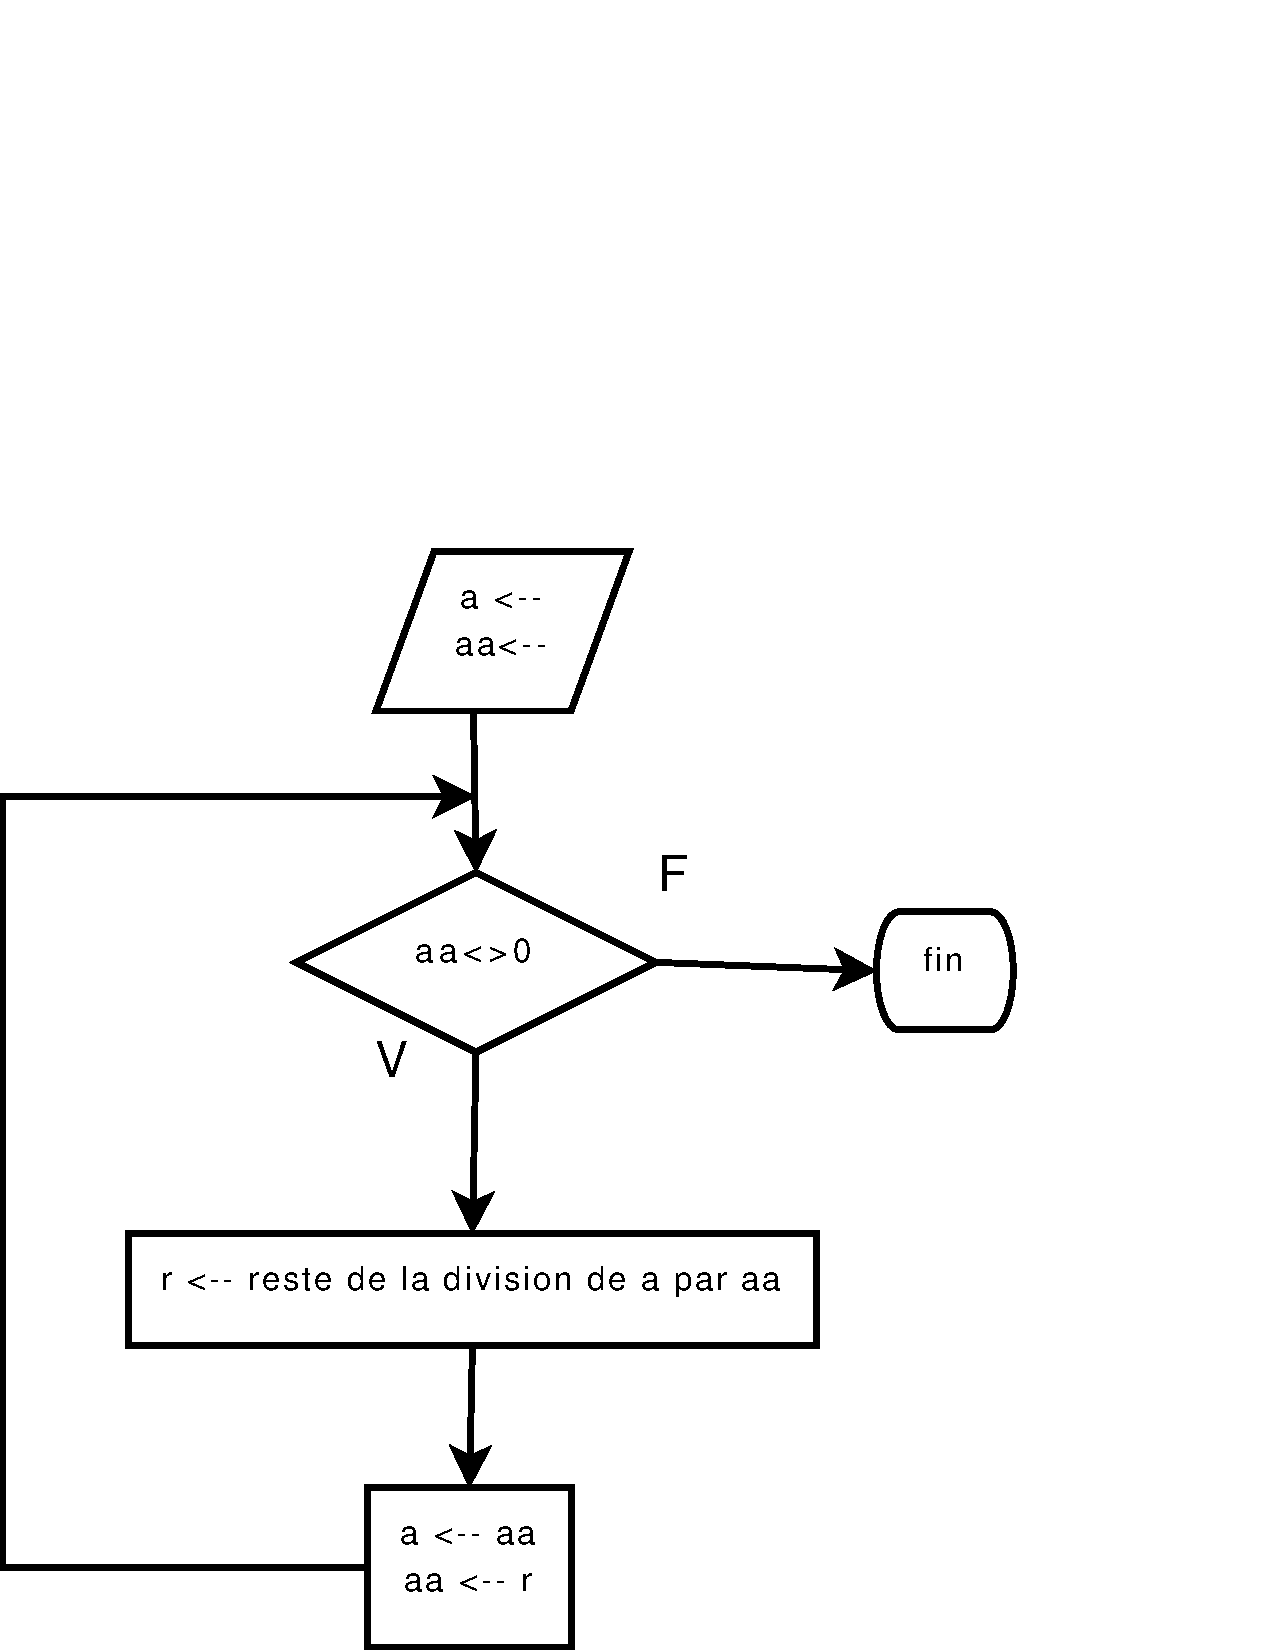
\includegraphics[width=9cm]{C5546_1.pdf}
 \caption{Algorithme "sec"}
 \label{C5546_1}
\end{figure}

\subsection{Calcul du pgcd - Existence de racines communes}
La présentation mathématique de ces algorithmes ainsi que la preuve du fonctionnement dans le cas étendu utilise les notations suivantes pour les divisions euclidiennes:
\begin{align*}
 a_0 &= q_1\,a_1 + a_2 \\
a_1 &= q_2\,a_2 + a_3 \\
   &\vdots \\
a_{n-2} &= q_{n-1}\,a_{n-1} +a_n\\
a_{n-1} &= q_n \, a_n
\end{align*}
L'élément $a_n$ est donc le dernier reste non nul. Le processus s'arrête car les valeurs absolues ou les degrés des $a_i$ sont strictement décroissants. \newline
On montre facilement que 
\begin{displaymath}
 \mathcal D (a_0)\cap \mathcal D (a_1) = \mathcal D (a_1)\cap \mathcal D (a_2) = \cdots = \mathcal D (a_{n-1})\cap \mathcal D (a_n) = \mathcal D (a_n) 
\end{displaymath}
car $a_n$ divise $a_{n-1}$. Ce qui prouve le résultat relatif au pgcd.
\begin{figure}[ht]
 \centering
 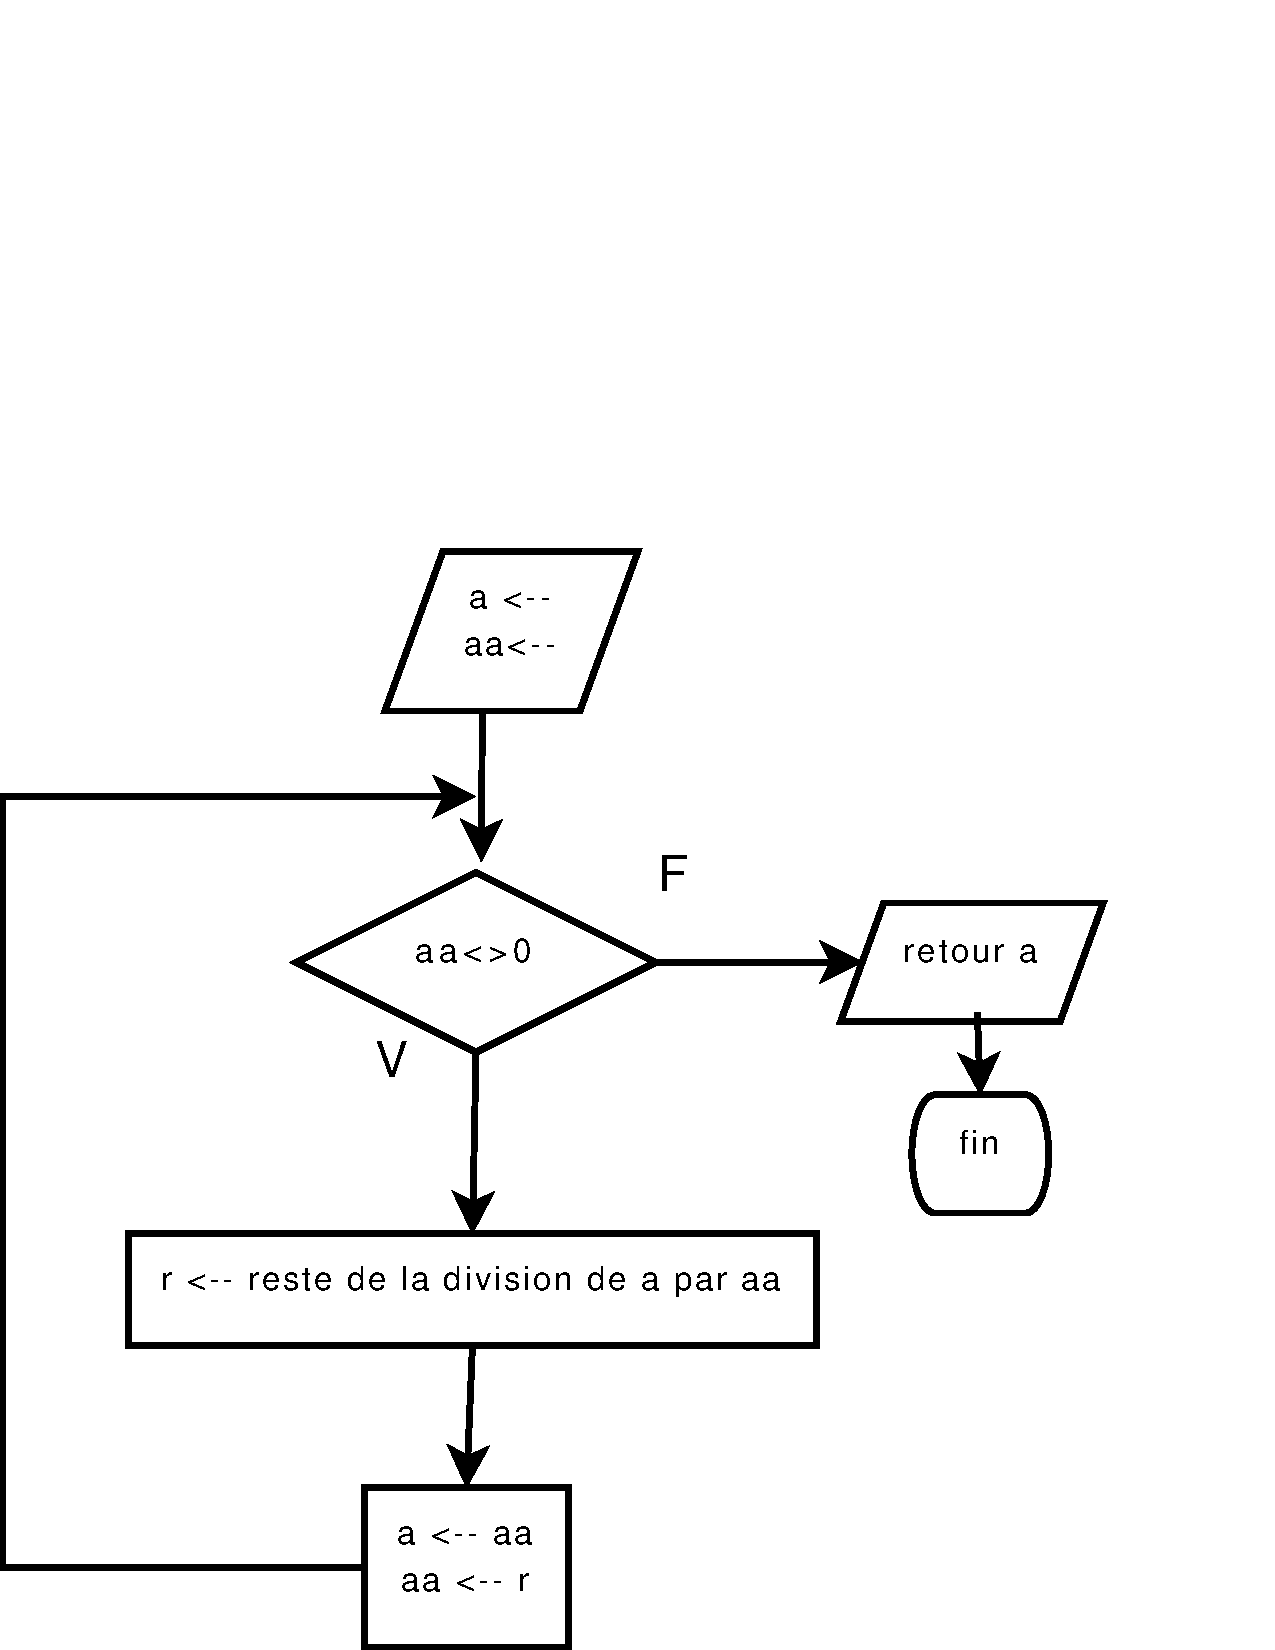
\includegraphics[width=10cm]{C5546_2.pdf}
 % C2160_1.pdf: 612x792 pixel, 72dpi, 21.59x27.94 cm, bb=0 0 612 792
 \caption{Calcul du pgcd}
 \label{C5546_2}
\end{figure}

\subsection{Algorithme d'Euclide étendu}
\index{algorithme d'Euclide étendu}
Il sert à calculer les coefficients permettant d'exprimer le dernier reste non nul en fonction des deux premiers termes de la suite. Il permet donc de résoudre pratiquement l'équation
\begin{displaymath}
 xa_0 + ya_1 =1
\end{displaymath}
 d'inconnue $(x,y)$ lorsque $a_0$ et $a_1$ sont premiers entre eux.\newline
Le principe est de considérer la relation de récurence définie par la suite des quotients $(q_1,q_2,\cdots,q_n)$. On dira qu'une famille $(x_0,x_1,\cdots,x_n)$ vérifie $\mathcal Q$ lorsque :
\begin{displaymath}
 (\mathcal Q)\hspace{2cm} \forall k\in\{2,\cdots,n\} : x_k = x_{k-2}-q_{k-1}x_{k-1}
\end{displaymath}
On remarque que la famille $(a_0,a_1,\cdots,a_n)$ vérifie $\mathcal Q$ car chaque relation traduit une des divisions euclidiennes. Considérons deux suites $(u_0,u_1,\cdots,u_n)$ et $(v_0,v_1,\cdots,v_n)$ vérifiant $\mathcal Q$ et définies par :
\begin{align*}
 u_0=1, u_1=0,  & & v_0=0, v_1=1
\end{align*}
Comme les trois familles $(a_0,a_1,\cdots,a_n)$ $(u_0,u_1,\cdots,u_n)$ et $(v_0,v_1,\cdots,v_n)$ vérifient $\mathcal Q$ et que :
\begin{align*}
 a_0 &= u_0a_0 + v_0a_1 \\
 a_1 &= u_1a_0 + v_1a_1
\end{align*}
Ces relations se propagent à tous les $k$ entre $2$ et $n$ et en particulier :
\begin{displaymath}
 a_n = u_na_0 + v_na_1
\end{displaymath}
Le diagramme de l'algorithme est modifié en introduisant de nouvelles variables u,uu,uuu,v,vv,vvv,q permettant de stocker les états des deux nouvelles suites et du quotient pour calculer les nouveaux termes.
\begin{figure}[ht]
 \centering
 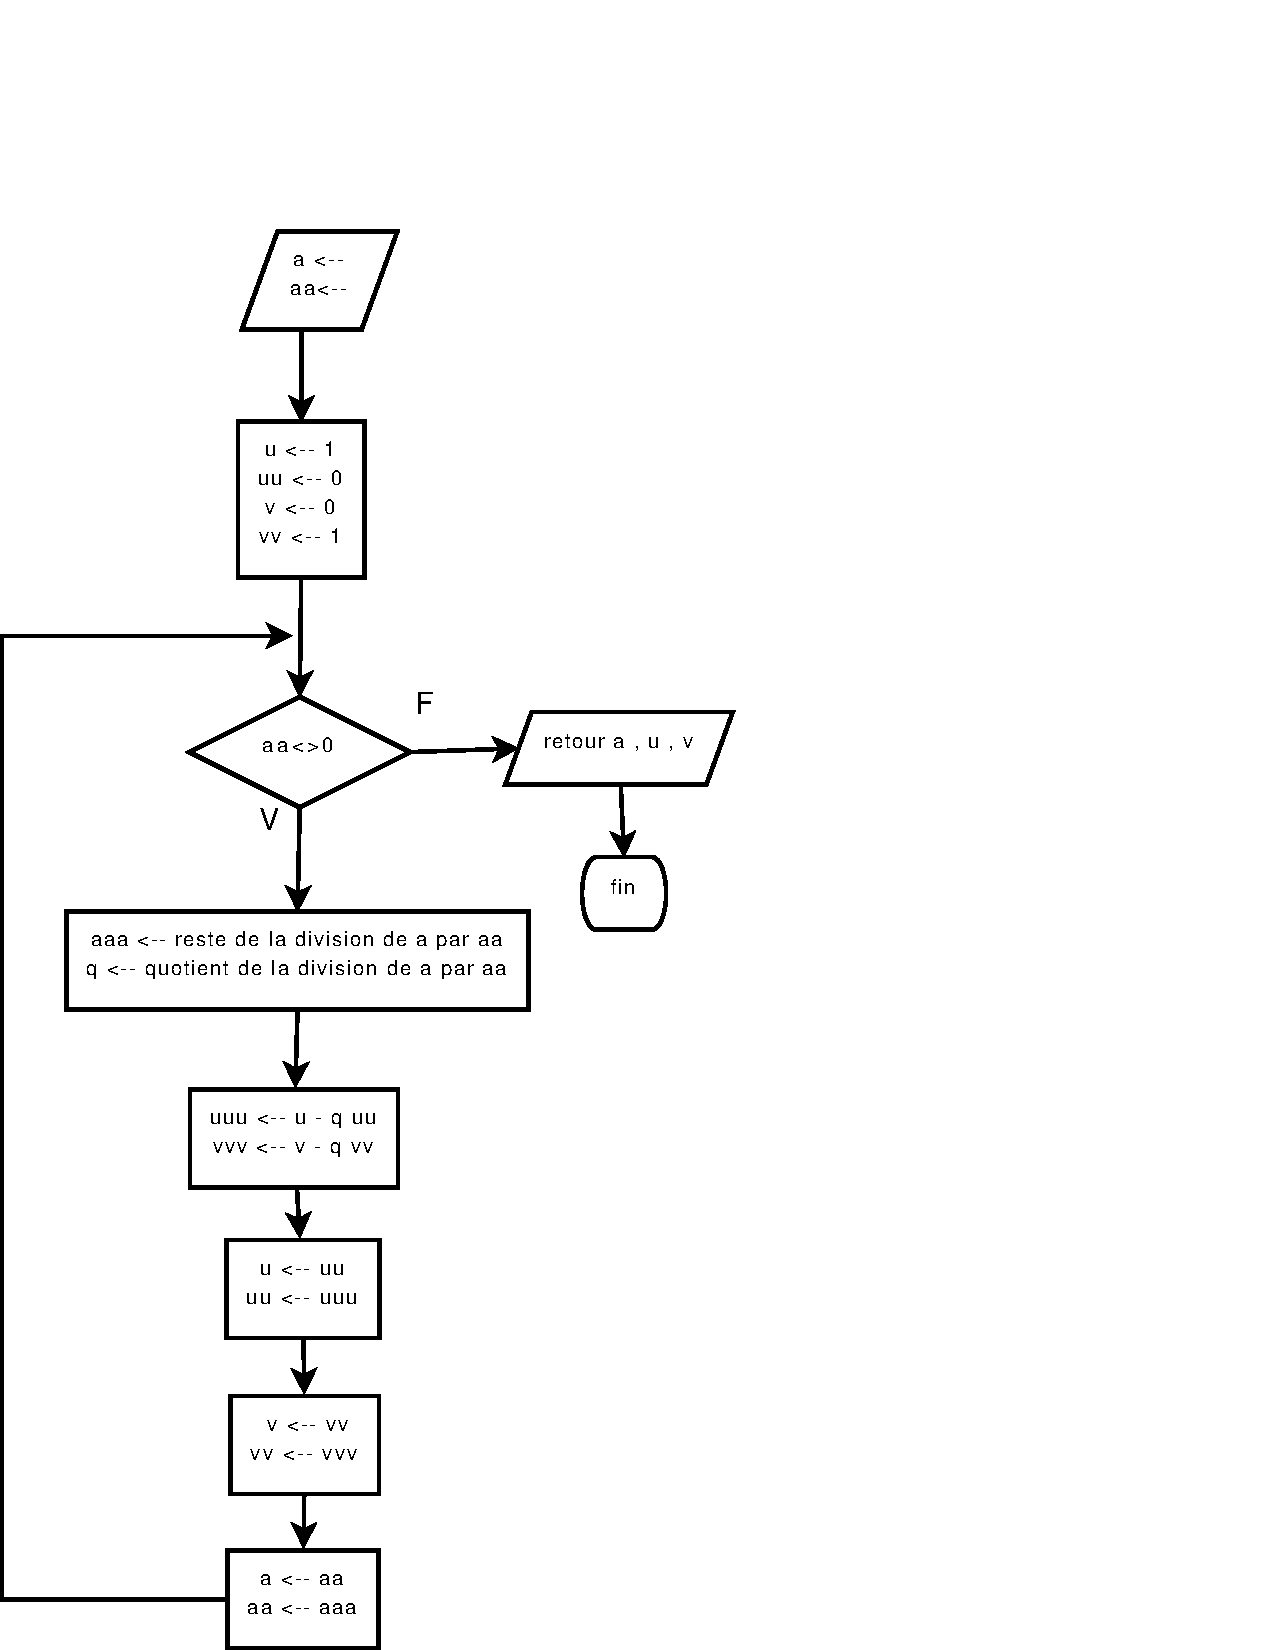
\includegraphics[width=12cm]{C5546_3.pdf}
 % C2160_1.pdf: 612x792 pixel, 72dpi, 21.59x27.94 cm, bb=0 0 612 792
 \caption{Algorithme dEuclide "étendu"}
 \label{C5546_3}
\end{figure}
\newline Pour un calcul "à la main", on peut utiliser une disposition en tableau \footnote{communiquée par Haitham Nasri}. Au début
\begin{displaymath}
% use packages: array
\begin{array}{l|l|l|l|l}
 & 0 & 1 & 2 & 3 \\ \hline
a & a_0 & a_1 & × & × \\ 
q & × & × & × & × \\ 
u & 1 & 0 & × & × \\
v & 0 & 1 & × & ×
\end{array}
\end{displaymath}
puis on progresse vers la droite avec chaque division euclidienne : d'abord $a_2$ et $q_1$, puis en utilisant la relation $\mathcal Q$,  $u_2$ et $v_2$ à partir des éléments de leur ligne respective et ainsi de suite
\begin{displaymath}
% use packages: array
\begin{array}{l|l|l|l|l}
 & 0 & 1 & 2 & 3 \\ \hline
a & a_0 & a_1 & a_2 & × \\ 
q & ×   & q_1 & ×   & × \\ 
u & 1   & 0   & 1 & × \\
v & 0   & 1   & -q_1 & ×
\end{array}
\hspace{1cm}\rightarrow\hspace{1cm}
\begin{array}{l|l|l|l|l}
 & 0 & 1 & 2 & 3 \\ \hline
a & a_0 & a_1 & a_2 & a_3 \\ 
q & ×   & q_1 & q_2   & × \\ 
u & 1   & 0   & 1 & -q_2 \\
v & 0   & 1   & -q_1 & 1+q_1q_2
\end{array}
\hspace{1cm}\rightarrow \hspace{1cm}\cdots
\end{displaymath}

\section{Divisibilité}
\subsection{Définitions}
\begin{prop}[Inversibles]
 L'ensemble des éléments inversibles de $\Z$ est $\{-1,+1\}$. L'ensemble des éléments inversibles de $\K[X]$ est $\K_0[X]\setminus\{0_{\K[X]}\}$ (ensemble des polynômes de degré $0$).
\end{prop}
 \begin{nota}
  On désigne par $\mathcal D (a)$ l'ensemble des diviseurs d'un élément $a$ non nul de $A$ et par $\mathcal M (a)$ l'ensemble de ses multiples. 
 \end{nota}
\begin{rem}
 Soit $a$ et $b$ deux éléments non nuls de $A$ alors $\mathcal M (a)\cap \mathcal M (b)$ est l'ensemble des multiples communs à $a$ et $b$ et $\mathcal D (a)\cap \mathcal D (b)$ est l'ensemble des diviseurs communs à $a$ et $b$  
\end{rem}

\begin{prop}
 Soit $a$ et $b$ deux éléments non nuls de $A$ qui se divisent mutuellement. Ils sont alors égaux à un  facteur inversible près. C'est à dire qu'il existe $c$ inversible tel que $b=ac$.
\end{prop}
\begin{rem}
  \begin{enumerate}
       \item  Soit $a$ et $b$ deux éléments non nuls de $A$ alors $\mathcal M (a)=\mathcal M (b)$ ou  $\mathcal D (a)=\mathcal D (b)$ si et seulement si $a$ et $b$ sont égaux à un facteur inversible près.
       \item Considérons une famille définie à un facteur inversible près. Lorsque $A=\Z$, il existe un seul élément de cette famille dans $\N$. Lorsque $A=\K[X]$, il existe un seul polynôme unitaire dans cette famille. En général ce sont ces éléments que l'on choisit pour représenter la famille.
   \end{enumerate}

\end{rem}

\begin{prop}[tout idéal est monogène]
 Soit $I$ une partie non vide de $A$ vérifiant les propriétés suivantes :
\begin{align*}
 \forall u\in A , \forall a\in I &: ua \in I \\
\forall a\in I , \forall b\in I &: a+b \in I 
\end{align*}
il existe alors un élément $m\in A$ unique à multiplication près par un inversible tel que $I = \mathcal M (m)$.
\end{prop}
\begin{demo}
 Utilise la division euclidienne. Cette démonstration est très proche de celle caractérisant les \href{\baseurl C2075.pdf}{sous-groupes de $(\Z,+)$}.
\end{demo}
\index{idéal}
\begin{rem}
 Une partie de $A$ vérifiant ces propriétés est appelée un \emph{idéal}\footnote{vocabulaire hors programme}.
\end{rem}


\subsection{PGCD. PPCM.}
\index{plus grand diviseur commun pgcd}\index{plus petit commun multiple ppcm}
\begin{defi}
 Soit $a$ et $b$ deux éléments non nuls de $A$.\\ Un \emph{plus grand commun dénominateur} (pgcd) de $a$ et $b$ est un élément $d$ tel que $\mathcal D(a)\cap \mathcal D(b)=\mathcal D(d)$.\\ Un \emph{plus petit commun multiple} (ppcm) de $a$ et $b$ est un élément $d$ tel que $\mathcal M(a)\cap \mathcal M(b)=\mathcal M(d)$.
\end{defi}
\begin{rem}
 Par définition, il n'y a pas d'unicité des pgcd et ppcm. Ils sont seulement uniques à un facteur inversible près. Si on impose de choisir des représentants particuliers (positifs pour $\Z$, unitaires pour $\K[X]$), on est assuré de l'unicité mais ce n'est pas toujours judicieux.
\end{rem}
\begin{nota}
 Soit $a$ et $b$ deux éléments non nuls de $A$. Le pgcd de $a$ est $b$ est noté $a\wedge b$ ou simplement $\text{pgcd}(a,b)$, le ppcm est noté $a\vee b$ ou simplement $\text{ppcm}(a,b)$.
\end{nota}
\begin{prop}
 Soit $a$ et $b$ deux éléments non nuls de $A$. Il existe des pgcd et des ppcm.
\end{prop}
\begin{demo}
 \begin{enumerate}
  \item Existence d'un pgcd (première méthode).\newline
On utilise l'algorithme d'Euclide avec $a_0=a$ et $b_0=b$. Si $a_n$ est le dernier reste non nul,
\begin{displaymath}
 \mathcal D(a_0) \cap\mathcal D(a_1)= \mathcal D(a_1) \cap\mathcal D(a_2)=\cdots = \mathcal D(a_{n-1}) \cap\mathcal D(a_n)=\mathcal D(a_n)
\end{displaymath}
ce qui assure que $a_n$ est un pgcd.
  \item Existence d'un ppcm.\newline
L'ensemble $\mathcal M (a)\cap \mathcal M (b)$ vérifie les hypothèses de la proposition \og tout idéal est monogène\fg. Cette proposition assure donc l'existence d'un ppcm.
 \item Existence d'un pgcd (deuxième méthode).\newline
 Soit $a$ et $b$ deux éléments non nuls de $A$. On désigne par $\mathcal M (a) + \mathcal M (b)$ l'ensemble des sommes d'un élément de $\mathcal M (a)$ et d'un élément de $\mathcal M (b)$. 
 Avec cette définition et celle des multiples, il est évident qu'un élément  $u\in A$ est dans $\mathcal M (a) + \mathcal M (b)$ si et seulement si il existe $x$ et $y$ dans $A$ tels que $u=xa+yb$. Il est immédiat aussi que $\mathcal M (a) + \mathcal M (b)$ vérifie les hypothèses de la proposition \og tout idéal est monogène\fg. On vérifie alors qu'un générateur de cet idéal est un pgcd ce qui constitue une deuxième preuve (non constructive) de l'existence.
 \end{enumerate}
\end{demo}
\begin{rems}
\begin{enumerate}
 \item D'après la proposition définissant le pgcd, il existe toujours des éléments $u$ et $v$ de $A$ tels que  $a\wedge b=ua +v b$.
 \item On peut étendre les définitions de pgcd et ppcm à des familles $(a_1,\cdots,a_p)$ de plus de deux éléments. Un pgcd de la famille est un élément $d$ vérifiant $\mathcal D(a_1)\cap\cdots \cap\mathcal D(a_p)=\mathcal D(d)$. Un ppcm de la famille est un élément $m$ vérifiant $\mathcal M(a_1)\cap\cdots \cap\mathcal M(a_p)=\mathcal M(d)$. Ces opérations (à un facteur inversible près) sont associatives car l'intersection est associative.
\end{enumerate}
 \end{rems}
\index{nombres premiers entre eux} \index{polynômes premiers entre eux}
\begin{defi}
 Deux éléments non nuls sont dits premiers entre eux lorsque leur pgcd est 1.
\end{defi}
\begin{rems}
\begin{enumerate}
 \item Deux éléments sont premiers entre eux si et seulement si l'ensemble de leurs diviseurs communs est l'ensemble des éléments inversibles.
 \item \index{éléments premiers entre eux dans leur ensemble} De même, les éléments d'un famille sont \emph{premiers entre eux dans leur ensemble} lorsque les inversibles sont leurs seuls diviseurs communs.
\end{enumerate} 
\end{rems}
\index{théorème de Bezout}
\begin{thm}[de Bezout]
 Soit $a$ et $b$ deux éléments non nuls de $A$.\newline
Il existe des éléments $u$ et $v$ dans $A$ tels que $au+bv$ soit un pgcd de $a$ et $b$. S'il existe des éléments $u$ et $v$ dans $A$ tels que $au+bv=1$ alors $a$ et $b$ sont premiers entre eux.
\end{thm}
\begin{demo}
 L'algorithme d'Euclide étendu constitue une première preuve de la première proposition qui est de plus constructive c'est à dire qu'elle donne un moyen pratique de déterminer $u$ et $v$. Cette première proposition est aussi une simple reformulation de la deuxième preuve (idéal somme) de l'existence d'un pgcd.\\
 S'il existe des éléments $u$ et $v$ dans $A$ tels que $au+bv=1$, il est immédiat que tout diviseur commun $d$ à $a$ et $b$ divise aussi $1$ c'est à dire qu'il est inversible.
\end{demo}

\index{théorème de Gauss}
\begin{thm}[de Gauss]
 Soit $a$, $b$, $c$ trois éléments non nuls de $A$ tels que $a$ divise $bc$ et $a$ premier avec $b$, alors $a$ divise $c$.
\end{thm}
\begin{rem}
 Une erreur fréquente consiste à supposer que $a$ ne divise pas $b$ au lieu de supposer que $a$ est premier avec $b$.
\end{rem}
\begin{demo}
 Comme $a$ est premier avec $b$, il existe $\lambda$ et $\mu$ dans $A$ tels que $\lambda a + \mu b=1$. Comme $a$ divise $bc$, il existe $u$ dans $A$ tel que $bc=ua$. On combine alors les deux relations :
\begin{displaymath}
 c=(\lambda a +\mu b)c - \mu(bc-ua)=(\lambda c +\mu u)a
\end{displaymath}
ce qui montre que $a$ divise $c$.
\end{demo}

\subsection{Compléments}
\subsubsection{Relations entre pgcd et ppcm}
Soit $I$ une partie de $A$ et $\lambda$ un élément non nul de $A$. On définit l'ensemble $\lambda I = \{\lambda a , a\in I\}$. On montre alors que 
\begin{align*}
 \mathcal M (\lambda a) &= \lambda \mathcal M ( a) \\
\mathcal M (\lambda a)\cap  \mathcal M (\lambda b) &= \lambda \left( \mathcal M ( a) \cap  \mathcal M (b)\right) \\
\mathcal M (\lambda a) + \mathcal M (\lambda b) &= \lambda \left( \mathcal M ( a) +  \mathcal M (b)\right)
\end{align*}
On en déduit alors que si $a$, $b$ et $\lambda$ sont des éléments non nuls de $A$ on a la propriété suivante (dite de linéarité du pgcd et du ppcm):
\begin{align*}
 \text{pgcd}(\lambda a, \lambda b)=\lambda \text{pgcd}(a, b) &,& \text{ppcm}(\lambda a, \lambda b)=\lambda \text{ppcm}(a, b)
\end{align*}
Dans la suite on note $d=\text{pgcd}(a,b)$ et $m=\text{ppcm}(a, b)$. Il existe alors des entiers $a^\prime$ et $b^\prime$ tels que $a=da^\prime$ et $b=db^\prime$. On se propose de montrer que
\begin{itemize}
 \item $a^\prime$ et $b^\prime$ sont premiers entre eux.
\item $md=ab$
\end{itemize}
Le premier point s'obtient par linéarité du pgcd.
\begin{displaymath}
 d=\text{pgcd}(a,b)=\text{pgcd}(da^\prime,db^\prime)=d\,\text{pgcd}(a^\prime,b^\prime)
\end{displaymath}
d'où $\text{pgcd}(a^\prime,b^\prime)=1$.\newline
Deux démonstrations sont proposées pour le second point 
\begin{displaymath}
 \text{pgcd}(a,b)\text{ppcm}(a,b)=ab
\end{displaymath}
\begin{demo}
 \begin{itemize}
 \item Remarquons que $ab$ est un multiple commun à $a$ et $b$ donc divisible par le ppcm. Introduisons $u$ par $ab=mu$ et montrons que $u$ est le pgcd de $a$ et $b$.\newline
Comme $a$ et $b$ divisent $m$, il existe $\alpha$ et $\beta$ tels que $m=\alpha b = \beta a$. On en déduit $a=u \alpha$ et $b=u \beta$ ce qui prouve que $u$ est un diviseur commun de $a$ et $b$.\newline
Utilisons maintenant la linéarité du ppcm :
\begin{displaymath}
 d^2 a^\prime b^\prime = ab=mu=\text{ppcm}(da^\prime,db^\prime)u=d\,\text{ppcm}(a^\prime,b^\prime)u
\end{displaymath}
On peut alors simplifier d'abord par $d$ puis par $\text{ppcm}(a^\prime,b^\prime)$ qui divise $a^\prime b^\prime$ ce qui entraîne que $d$ divise $u$.
\item Une autre manière de procéder est de montrer directement que $da'b'=\text{ppcm}(a,b)$.\newline
Remarquons d'abord que $da'b'=ab'=a'b$ est un multiple commun à $a$ et $b$. On sait donc que $m=\text{ppcm}(a,b)$ divise $da'b'$.\newline
D'autre part, $m$ est un multiple commun, il existe donc $\lambda$ et $\mu$ dans $A$ tels que 
\begin{displaymath}
m=\lambda a = \mu b \Rightarrow \lambda a' = \mu b' 
\end{displaymath}
après simplification par $d$. Donc $a'$ divise $\mu b'$ en étant premier avec $b'$ ce qui entraine que $a'$ divise $\mu$ (Thèorème de Gauss). Il existe donc $k\in A$ tel que
\begin{displaymath}
 \mu = k a' \Rightarrow  \lambda a' =  k a'b' \Rightarrow \lambda = kb' 
\Rightarrow m = k b' a = k da' b'
\end{displaymath}
Ce qui prouve que $da'b'$ divise $m$ et achève la démonstration.
\end{itemize}
\end{demo}


Une conséquence de ce que l'on vient de montrer est que deux éléments sont premiers entre eux si et seulement si leur ppcm est égal à leur produit.

\subsubsection{\'Etude de l'équation de Bézout.}
\index{équation de Bezout}
Il s'agit de l'équation
\begin{displaymath}
 au+bv=c
\end{displaymath}
où $a$, $b$, $c$ sont des paramètres dans $A$ et les inconnues sont $u$ et $v$. On supposera que $a$ et $b$ sont non nuls et non inversibles. Les points à retenir sont :
\begin{itemize}
 \item L'équation admet des solutions si et seulement si $c$ est un multiple du pgcd de $a$ et de $b$.
\item Lorsque $c$ est un multiple de du pgcd de $a$ et $b$, on peut tout simplifier par ce pgcd et se ramener ainsi au cas où $a$ et $b$ sont premiers entre eux.
\item Lorsque $a$ et $b$ sont premiers entre eux on peut préciser l'ensemble des couples solutions en fonction d'un couple solution particulier. Si $(u_0,v_0)$ est une solution particulière, l'ensemble des solutions est:
\begin{displaymath}
 \left\lbrace (u_0-\lambda b, v_0+\lambda a),\lambda \in A\right\rbrace 
\end{displaymath}
Une inclusion est évidente, l'autre se démontre à l'aide du théorème de Gauss.
\item On peut trouver un couple solution en utilisant l'algorithme d'Euclide étendu.
\item Lorsque $a$ et $b$ sont premiers entre eux et que $c=1$, il existe un couple particulier de "petites" solutions. Le mot est à préciser suivant que $A=\Z$ ou $\K[X]$. Ce couple est unique dans le cas où $a$ et $b$ sont premiers entre eux.\begin{itemize}
 \item Dans le cas de $\Z$, on suppose $a$ et $b$ supérieur ou égal à $2$. Il existe un unique couple solution $(u_1,v_1)$ tel que $0<u_1<b$ et $0<-v_1<a$
\item Dans le cas de $\K[X]$, il existe un unique couple solution $(u_1,v_1)$ tel que $\deg u_1 < \deg b$ et $\deg v_1<\deg a$.
\end{itemize}
L'existence se prouve par une division euclidienne de $u_0$ par $b$ lorsque $(u_0,v_0)$ est une solution particulière. On note $u_1$ le reste, il existe alors une solution $(u_1,v_1)$. La condition sur $v_1$ se verifie en considérant $bv_1 = 1- au_1$ et en formant des inégalités (pour le degré dans le cas de $\K[X]$).
\end{itemize}


\section{Nombres premiers. Polynômes irréductibles}
\index{polynôme irréductible}
\begin{defi}[polynôme irréductible]
 Un polynôme $P\in \K[X]$ est dit \emph{irréductible} si et seulement si il est de degré au moins $1$ et ses seuls diviseurs sont inversibles ou de la forme $\lambda P$ avec $\lambda$ élément non nul de $\K$. 
\end{defi}
\index{nombre premier}
\begin{defi}[nombre premier]
 Un entier naturel $a$ est dit \emph{premier} si et seulement si il est supérieur ou égal à $2$ et ses seuls diviseurs sont $1$, $-1$, $a$, $-a$.
\end{defi}
\begin{prop}
 Tout élément non nul $a$ de $A$ admet un diviseur premier (cas de $\Z$) ou irréductible (cas de $\K[X]$).
\end{prop}
\begin{demo}
 On considère l'ensemble formé par les valeurs absolues ou les degrés des diviseurs de $a$. C'est une partie non vide de $\N$, elle admet don un plus petit élémént. Soit $p$ un élément de $A$ dont la valeur absolue ou le degré est égal à ce plus petit élément, on vérifie facilement que $p$ est premier ou irréductible. 
\end{demo}
\begin{prop}
 Soit $a$ un élément non nul et non inversible de $A$, et $p_1, p_2, \cdots, p_n$ des diviseurs de $a$ deux à deux premiers entre eux, alors $p_1p_2\cdots p_n$ divise $a$.
\end{prop}
\begin{demo}
 récurrence sur $n$ à rédiger à base de thm de Gauss.
\end{demo}
\begin{nota}
L'ensemble des diviseurs (premiers ou irréductibles) d'un élément $a$ non inversible est non vide et fini. Il est noté $\mathcal D_p(a)$. 
\end{nota}
\begin{prop}
L'ensemble des nombres premiers n'est pas fini. 
\end{prop}
\begin{defi}
 Supposons que $p_1<p_2<\cdots<p_n$ soient $n$ nombres premiers  et considérons $a=p_1p_2\cdots p_n+1$. D'après le théorème de Bezout cet élément est premier avec les $p_i$. Il admet donc un diviseur premier autre que les $p_i$ qui ne peuvent donc constituer à eux seuls l'ensemble de tous les nombres premiers. 
\end{defi}
\index{décomposition en facteurs premiers}\index{décomposition en facteurs irréductibles}
\begin{prop}[décomposition en facteurs premiers ou irréductibles]
Tout élément $a$ non inversible est produit d'éléments premiers ou irréductibles. 
 Il existe  $u$ inversible, $p_1,\cdots p_k$ premiers ou irréductibles unitaires deux à deux distincts et $\alpha_1,\cdots,\alpha_k$ entiers $\geq 1$ tels que
\begin{displaymath}
 a = u p_1^{\alpha_1} \cdots p_k^{\alpha_k} 
\end{displaymath}
Une telle écriture est unique à permutation près sur les indices $i$ entre $1$ et $k$.
\end{prop}
\begin{demo}
 L'existence de la décomposition repose sur un raisonnement par récurrence portant sur la valeur absolue ou le degré. La démonstration de l'unicité repose d'abord sur le théorème de Gauss. Elle n'est pas détaillée ici.
\end{demo}
\begin{rem}
Pour chaque diviseur $p$ (premier ou irréductible) de $a$, il existe un unique entier $m_a(p)\geq 1$ tel que 
\begin{displaymath}\left\lbrace 
\begin{aligned}
 p^{m_a(p)} &\text{ divise } a\\
 p^{m_a(p)+1} &\text{ ne divise pas } a
\end{aligned}\right. 
\end{displaymath}
Lorsque $p$ n'est pas un diviseur de $a$, on pose $m_a(p)=0$ de sorte que, en désignant par $\mathcal P$ l'ensemble des nombres premiers ou des irréductibles unitaires, la décomposition peut s'écrire
\begin{displaymath}
 a=\lambda\prod_{p\in \mathcal P}p^{m_a(p)}
\end{displaymath}
étant entendu que ce produit est en fait fini car les $m_p(a)$ sont nuls sauf pour un nombre finis de $p$.\newline
Il est intéressant de remarquer que:
\begin{displaymath}
 \forall p\in \mathcal P :\; m_p(a\wedge b)=\min(m_p(a),m_p(b))\hspace{1cm}m_p(a\vee b)=\max(m_p(a),m_p(b))
\end{displaymath}
 ce qui, avec 
\begin{displaymath}
m_p(a\wedge b)=m_p(a)+m_p(b)= \min(m_p(a),m_p(b))+ \max(m_p(a),m_p(b))
\end{displaymath}
redonne $(a\wedge b)(a\vee b)=ab$.
\end{rem}
  
\end{document}